\documentclass[11pt]{article}
\usepackage[margin=2cm]{geometry}
\usepackage{booktabs,graphicx,amsmath,amssymb,xcolor,enumitem,hyperref}
\usepackage[T1]{fontenc}
\usepackage{lmodern}
\hypersetup{colorlinks,linkcolor=blue!50!black,urlcolor=blue!50!black}
\setlist{itemsep=1pt,topsep=3pt}
\newcommand{\code}[1]{\texttt{#1}}
\newcommand{\ours}[1]{\textcolor{blue!60!black}{\textbf{#1}}}
\newcommand{\naive}[1]{\textcolor{orange!70!black}{#1}}
\setlength{\parindent}{0pt}\setlength{\parskip}{4pt}

\title{\vspace{-1.2cm}A kernel-writing agent under an 8k-token budget\\[2pt]\large Demo notes, Team 27 (seat 130) \textbullet{} Project 02, Stage A}
\date{2026-10-10 \textbullet{} \href{https://github.com/yahavb/trainium-agent-labs/pull/20}{PR \#20}: \code{projects/team-27-kernel-agent/} in the fork \url{https://github.com/LiYou22/trainium-agent-labs} (branch \code{team-27-kernel-agent})}
\author{}

\begin{document}
\maketitle
\vspace{-1cm}

\section*{1. The problem and our claim}
Qwen3-8B (vLLM on a Trainium seat pod, 8192 tokens per call including the answer) must write tiled
NumPy kernels for a 10-level ladder (relu \dots\ conv1d) under chip-like rules: tiles of at most
$128\times512$, explicit loops, no fancy indexing or broadcasting, no calling the op itself, partial
tiles handled. The dilemma: rules in the prompt make the small model audit itself into silence; no
rules and it writes confident violations (our first L1 kernel: 40/40 correct, but \code{np.asarray}
on line 5, so zero).

\textbf{Claim: the rules belong in the verifier, not the prompt; every verdict is translated into one
concrete instruction.} The model writes freely from a one-sentence task; the harness finds what is
wrong; the agent sends back the previous code, \emph{one} instruction and one line of evidence; a
kernel counts only if it also passes held-out cases the model never saw.

\section*{2. The verifier}
\begin{itemize}
\item \textbf{Two rule checks}: a static AST scan (covers branches the tests never reach) and a runtime
  guard (numpy swapped for a monitored proxy that records each violation by line).
\item \textbf{Numerical correctness} against a proven float32 error bound (\S5), on hostile dev cases
  (huge magnitudes, large means, partial tiles) and a separate holdout set.
\item \textbf{Diagnosis, not just a verdict}: cross-case patterns (``wrong exactly when there is more
  than one column tile''), and level hypotheses checked numerically against the reference before they
  are said (a wrong explanation is worse than none).
\item \textbf{Cost ledger}: FLOPs, instructions, HBM bytes read/written for every run (\S6).
\item \textbf{Final gate}: the organizers' \code{kernelbench.py}; its failures are translated too.
\end{itemize}

\section*{3. Key result: final agent vs naive}
\ours{Ours} = the final agent (version \code{c5e98d5a75}); \naive{naive} = the same verifier and model, but
the verifier's report is sent back verbatim instead of being translated into one instruction
(\code{e22ccab872}). Holdout and stopping rule are the same. Reward per run = best attempt: 0.1 parses
+ 0.2 obeys rules + 0.2 runs + 0.5 $\times$ fraction of cases correct (the upstream NKI agent's formula).

\begin{center}\small
\begin{tabular}{@{}lcccc@{}}\toprule
Level & solved (ours / naive) & per-run reward, ours & per-run reward, naive & mean reward \\\midrule
L1 relu & \ours{5/5} / \naive{3/5} & 1.00 1.00 1.00 1.00 1.00 & 0.80 0.80 1.00 1.00 1.00 & \ours{1.00} / \naive{0.92}\\
L2 row sum & \ours{3/3} / \naive{0/5} & 1.00 1.00 1.00 & 0.80 0.80 0.80 0.80 0.80 & \ours{1.00} / \naive{0.80}\\
L3 row max & \ours{3/3} / \naive{1/5} & 1.00 1.00 1.00 & 1.00 0.80 0.81 0.80 0.80 & \ours{1.00} / \naive{0.84}\\
L4 RMSNorm & \ours{0/4} / \naive{0/5} & 0.81 0.81 0.81 0.61 & 0.74 0.61 0.61 0.61 0.74 & \ours{0.76} / \naive{0.66}\\
L5 softmax & \ours{3/4} / \naive{0/5} & 1.00 0.67 1.00 1.00 & 0.80 0.47 0.80 0.47 0.80 & \ours{0.92} / \naive{0.67}\\
L6 transpose & \ours{3/3} / \naive{1/5} & 1.00 1.00 1.00 & 0.80 0.80 0.80 0.80 1.00 & \ours{1.00} / \naive{0.84}\\
L7 matmul & \ours{1/2} / \naive{0/5} & 1.00 0.83 & 0.80 1.00 1.00 1.00 0.80 & \ours{0.92} / \naive{0.92}\\
L8 layernorm & \ours{1/5} / \naive{0/5} & 1.00 0.61 0.73 0.61 0.94 & 0.80 0.80 0.61 0.61 0.61 & \ours{0.78} / \naive{0.69}\\
L9 band attention & \ours{4/5} / \naive{0/5} & 1.00 1.00 1.00 0.58 1.00 & 0.80 0.80 0.52 0.80 0.80 & \ours{0.92} / \naive{0.74}\\
L10 conv1d & \ours{1/2} / \naive{4/5} & 1.00 0.35 & 1.00 0.10 1.00 1.00 1.00 & \ours{0.68} / \naive{0.82}\\
\midrule
\textbf{Total} & \ours{24/36} / \naive{9/50} & & & \ours{0.90} / \naive{0.79}\\
\bottomrule
\end{tabular}\end{center}
\vspace{-4pt}{\footnotesize The final agent's runs were still in progress at 18:35 (completed runs only,
hence 2--5 per level).}

Naive's many 0.80s are numerically right but rule-breaking (e.g.\ \code{np.sum}): given the raw report,
the model repeats the same mistake. Tokens per solved kernel: \ours{8.6k} vs \naive{25.2k}, about
$3\times$ cheaper per success. Not every level improves: naive is better on L10, and L4 is unsolved.

\textbf{One failure and its recovery (L2, live log).} \#1 uses \code{np.sum}: 28/28 correct but illegal
$\to$ ``accumulate column by column, \code{acc += x[i0:i1, j]}''. \#2 column loop, but indexes a 188-column
partial tile with the global column: \code{IndexError: index 512 is out of bounds for axis 1 with size 188}
(19/28 cases crash) $\to$ one instruction about the partial tile. \#3 dev 28/28, holdout 21/21.

\textbf{One new diagnosis (L3).} The live bug \code{result[row] = acc} sat inside the column-tile loop,
so each tile overwrote the last. The verifier now recomputes the reference per tile, sees the wrong
outputs equal the last tile's result, and says ``keep one running value per row across all tiles;
write it after the loop''. L3 went from stuck to 5/5.

\section*{4. Final kernel per level}
Each written by the agent and passing \emph{both} our checker (rules, dev, holdout) and the organizers'
\code{kernelbench.py} (\code{FINAL.md}, \code{kernels/final/}):

\begin{center}\small
\begin{tabular}{@{}lcccccccccc@{}}\toprule
 & L1 & L2 & L3 & L4 & L5 & L6 & L7 & L8 & L9 & L10\\\midrule
both checkers & \checkmark & \checkmark & \checkmark & -- & \checkmark & \checkmark & -- & \checkmark & \checkmark & \checkmark\\
roofline time & 1.00 & 1.00 & 1.00 & & 2.00 & 1.00 & & 2.00 & 61.2 & 12.2\\\bottomrule
\end{tabular}\end{center}

\section*{5. Numerical analysis: bound the error, don't guess a tolerance}
An output passes iff $|y - y_\text{ref}| \le \gamma_k \cdot \text{scale}$ with
$\gamma_k = ku/(1-ku)$, $u = 2^{-24}$ (Higham), $k$ the longest chain of roundings (row length for a
sum, $K$ for matmul, the window for attention/conv), scale the op's natural magnitude (e.g.\
$\sum|x|$ for a row sum). Any algorithm correct in float32 passes, whatever its order; bugs still
fail by orders of magnitude.

\begin{center}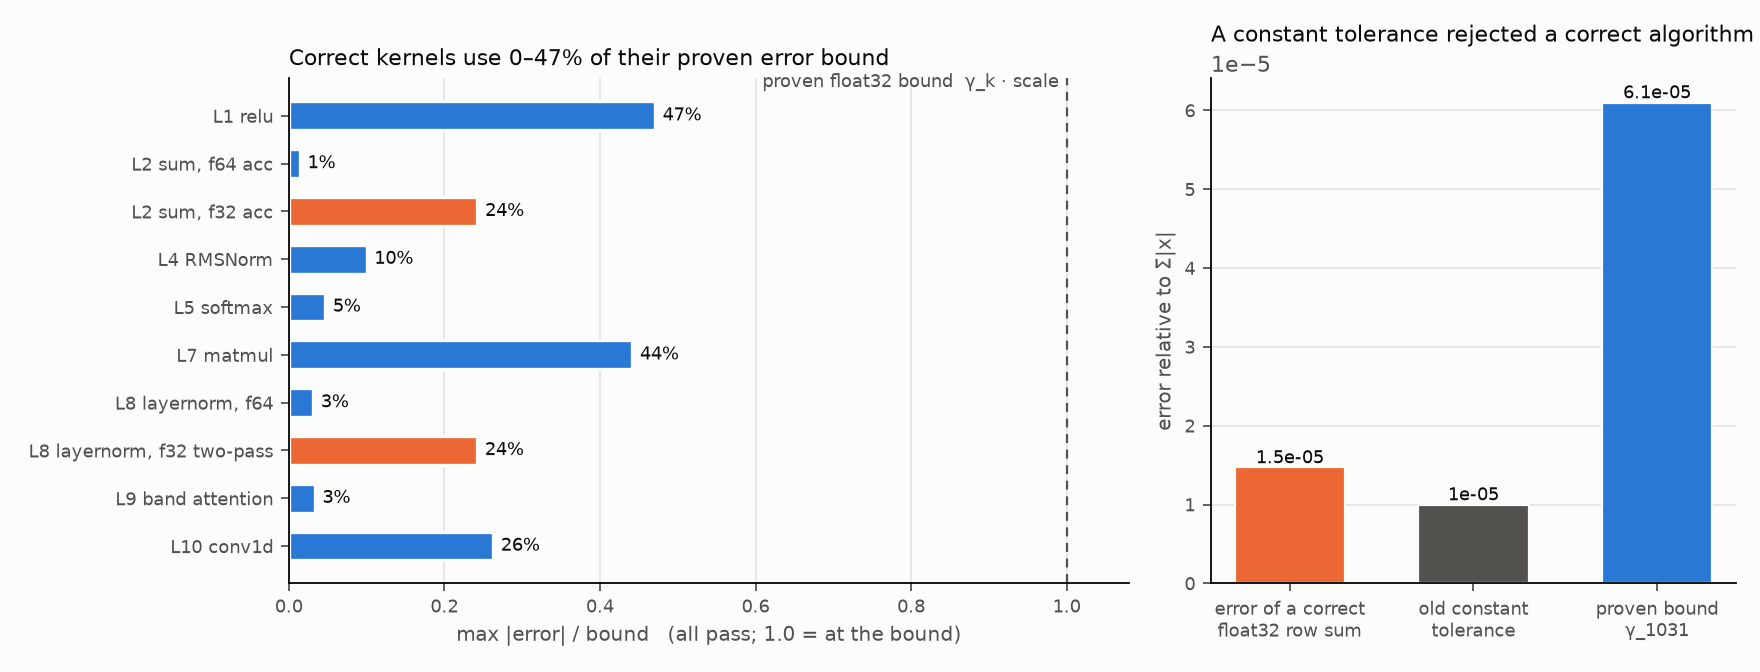
\includegraphics[width=0.92\linewidth]{fig-bounds.png}\end{center}
\vspace{-6pt}Our first constant tolerance ($10^{-5}$) rejected a \emph{correct} float32 row sum
(error $1.5\times10^{-5}$; proven bound $6.1\times10^{-5}$). All hand kernels use 0--47\% of their bound.

\section*{6. Efficiency: count FLOPs, bytes and instructions}
The runtime guard keeps books for every run: FLOPs, instructions (numpy calls, including scalar ops),
HBM bytes read and written, each against the op's minimum. Cost is the roofline time
$t=\max(\text{HBM bytes}, \text{FLOPs}/222)$ as a multiple of the minimum (222 FLOP/byte is the ridge).
These ops run at 0.25--0.44 FLOP/byte, so they are memory-bound: the win is fewer passes and
instructions, not fewer FLOPs.

\begin{center}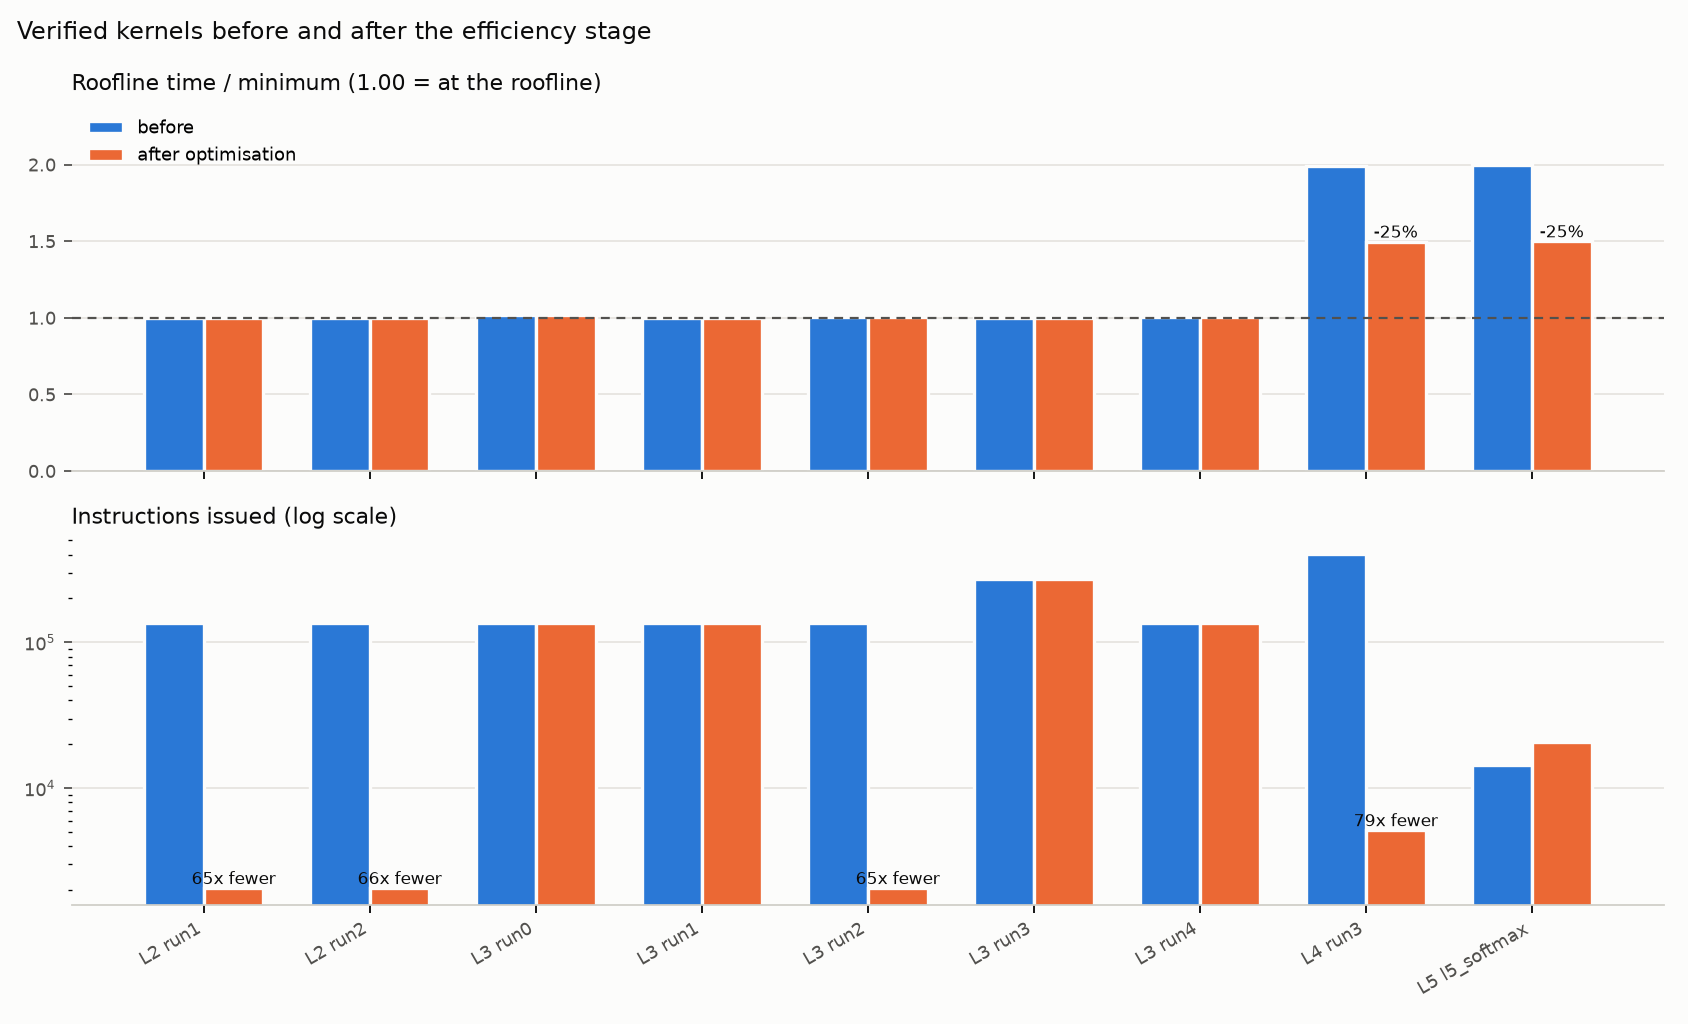
\includegraphics[width=0.78\linewidth]{fig-opt2.png}\end{center}
\vspace{-6pt}8 of 15 verified model kernels were per-element loops ($\sim$135k instructions where
column vectors need 2{,}068), all ``correct''. The optimiser gives one rule-safe instruction with a
snippet and accepts a rewrite only if dev \emph{and} holdout still pass and it is cheaper:
\textbf{65$\times$ / 79$\times$ fewer instructions}, L4 roofline $1.99\times \to 1.50\times$; no kernel
was ever made wrong.

\section*{7. Honest limits}
\begin{itemize}
\item L4 and up are still hard: two passes + no broadcasting + numeric traps; fixing one breaks another.
  L4 and L7 have no kernel passing both checkers.
\item Samples are small (2--5 runs per level) and the server is near-deterministic, so each run uses a
  different wording of the task.
\item The 8k budget never bound in Stage A (largest prompt 706 tokens); it would in Stage B (NKI).
\end{itemize}

\section*{8. Demo instructions (about 3 minutes, no model needed)}
{\footnotesize
\begin{verbatim}
git clone -b team-27-kernel-agent https://github.com/LiYou22/trainium-agent-labs.git
cd trainium-agent-labs/projects/team-27-kernel-agent && uv sync
export KERNELBENCH_DIR=$PWD/../02-kernel-agent   # organizers' kernelbench.py, in the same repo

# (a) the verifier names the cause, not just "wrong"                          -> Sec. 3, L3
uv run python -m kagent.harness 3 kernels/broken/l3_overwrite_per_tile.py --fixes
# (b) a rule violation becomes ONE instruction                                -> Sec. 3, L2
uv run python -m kagent.harness 2 kernels/broken/l2_np_sum.py --fixes
# (c) error bound and cost ledger on a correct kernel                         -> Sec. 5, 6
uv run python -m kagent.harness 4 kernels/hand/l4_rmsnorm.py
# (d) the full repair loop, replaying recorded model replies                  -> Sec. 1, 3
uv run python -m kagent.agent --levels 1 2 --scripted tests/scripts/demo.json --out /tmp/demo.jsonl
# (e) the per-run rewards of the ablation table                               -> Sec. 3
uv run python scripts/reward.py results/seat-130/ours-L1234-seat-130.jsonl \
                                results/seat-130/naive-L1234-seat-130.jsonl
\end{verbatim}
}
\begin{description}[leftmargin=0pt,itemsep=3pt]
\item[(a) The verifier names the cause.] A kernel the model really wrote for L3 (row max) with
  \code{result[row] = acc} inside the column-tile loop. Point at \code{0 rule violation(s), 15/24 cases
  correct}: no rule broken, 9 cases wrong. The verifier does not stop at ``wrong'': \code{Pattern: \dots\
  each wrong output equals the result over the last column tile only} names the bug (each tile
  overwrites the last), which is what lets the model fix it (\S3, L3).
\item[(b) A violation becomes one instruction.] An L2 (row sum) kernel calling \code{np.sum}. Point at
  \code{28/28 cases correct} \emph{and} \code{np.sum [sum-like]}: numerically right, still a failure,
  because it calls the op it must implement. \code{--fixes} prints the one instruction the agent
  sends: \code{FIX line 12: Replace np.sum with an explicit python loop over the columns \dots}
  (\S3, step 1 of the L2 recovery).
\item[(c) Error bound and cost ledger.] Our correct hand RMSNorm. Point at \code{worst uses 10\% of it}:
  the largest error is 10\% of the proven float32 bound (\S5); and at the \code{Cost} line: FLOPs, HBM
  reads/writes and instructions against the op's minimum (\S6).
\item[(d) The whole loop.] The real agent loop, with recorded model replies instead of live calls, so
  it takes seconds and needs no server. In L2: the model's code uses \code{np.sum} $\to$ \code{FAIL
  rule:sum-like} $\to$ one instruction $\to$ \code{PASS dev; holdout 21/21} $\to$ \code{verified
  (confidence 0.95)}; 0.95 means it also passed the organizers' checker. \code{in=}/\code{out=} on each
  line are the tokens of that call.
\item[(e) The table comes from the logs.] Reads the real seat-130 run logs of both arms and prints each
  level's per-run reward: the same numbers as the table in \S3, computed, not typed.
\end{description}
Order: (a) and (b) show how the verifier finds a problem and turns it into one instruction; (c) shows
the numerical analysis and the cost ledger; (d) ties them into the loop; (e) shows the results are
traceable. Self-tests: \code{uv run pytest -q} (74 passed); \code{README.md} has the commands for live runs.

\end{document}
